\documentclass{beamer}
\usepackage[utf8]{inputenc}
\usepackage[T1]{fontenc}

\usetheme{focus}
\definecolor{main}{RGB}{11, 93, 25}

\usecolortheme[RGB={11,93,20}]{structure}
\usepackage[spanish]{babel}

\usepackage{colortbl}
\usepackage{color}
\usepackage{pifont}
\usepackage{ulem}



\author{Alberto Molina Coballes}
\title{El kérnel del sistema operativo}
\institute{IES Gonzalo Nazareno}
\titlegraphic{
\includegraphics[width=1.5cm]{cc_by_sa.png}}
\logo{
\includegraphics[width=.75cm]{logo_iesgn.png}}
\date{\today}

\definecolor{verde}{rgb}{0,0.73,0}

\begin{document}
\begin{frame}[t,plain]
\titlepage
\end{frame}

\begin{frame} \frametitle{Funciones del kérnel}
  \begin{itemize}
  \item El kérnel (núcleo) es la parte fundamental del sistema
    operativo y se encarga de manejar los recursos y permitir que los
    programas hagan uso de los mismos, siendo los principales recursos:
    \begin{itemize}
    \item CPU
    \item Memoria
    \item Dispositivos de Entrada/salida
    \end{itemize}
  \item Además el kérnel es el encargado proporcionar:
    \begin{itemize}
    \item Protección mediante diferentes niveles de acceso
    \item Acceso compartido (multiplexado) a los recursos
    \end{itemize}
  \end{itemize}
\end{frame}

\begin{frame} \frametitle{Niveles de seguridad}
  \begin{columns}
    \column{0.6\textwidth}
    \begin{itemize}
    \item Algunas CPU incluyen diferentes niveles de acceso, que se
      conocen como anillos (\emph{rings}).
    \item Los diferentes kérnel suelen utilizar al menos dos niveles
      para acceder tanto a la CPU como a la memoria:
      \begin{itemize}
      \item kernel mode (Sin restricciones)
      \item user mode (Restringido)
      \end{itemize}
    \end{itemize}
    \column{0.35\textwidth}
    \begin{center}
      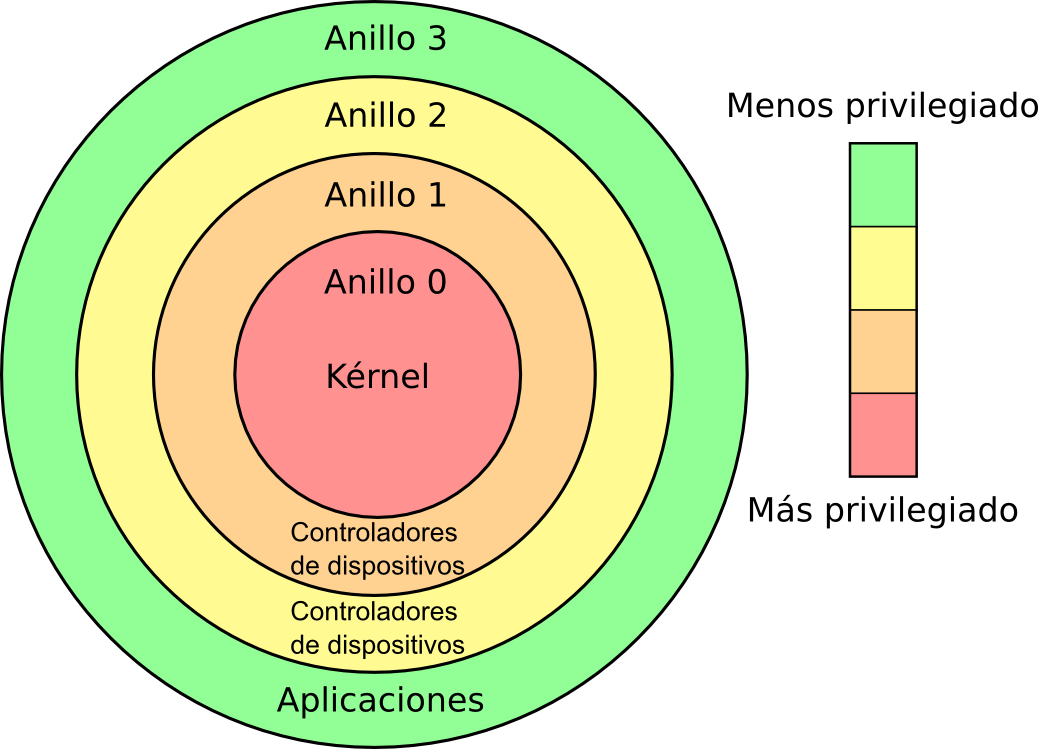
\includegraphics[width=\columnwidth]{Priv_rings.png}
    \end{center}
  \end{columns}
    \begin{itemize}
    \item kernel monolítico: Todo en kernel mode
    \item FUSE: Filesystem in User Space (sshfs, ntfs-3g, ...)
    \item CUSE: Character devices in User Space
    \end{itemize}
    \footnotesize{\url{https://en.wikipedia.org/wiki/Protection_ring}}
\end{frame}

\begin{frame} \frametitle{Tipos de kérnel}
  \begin{center}
  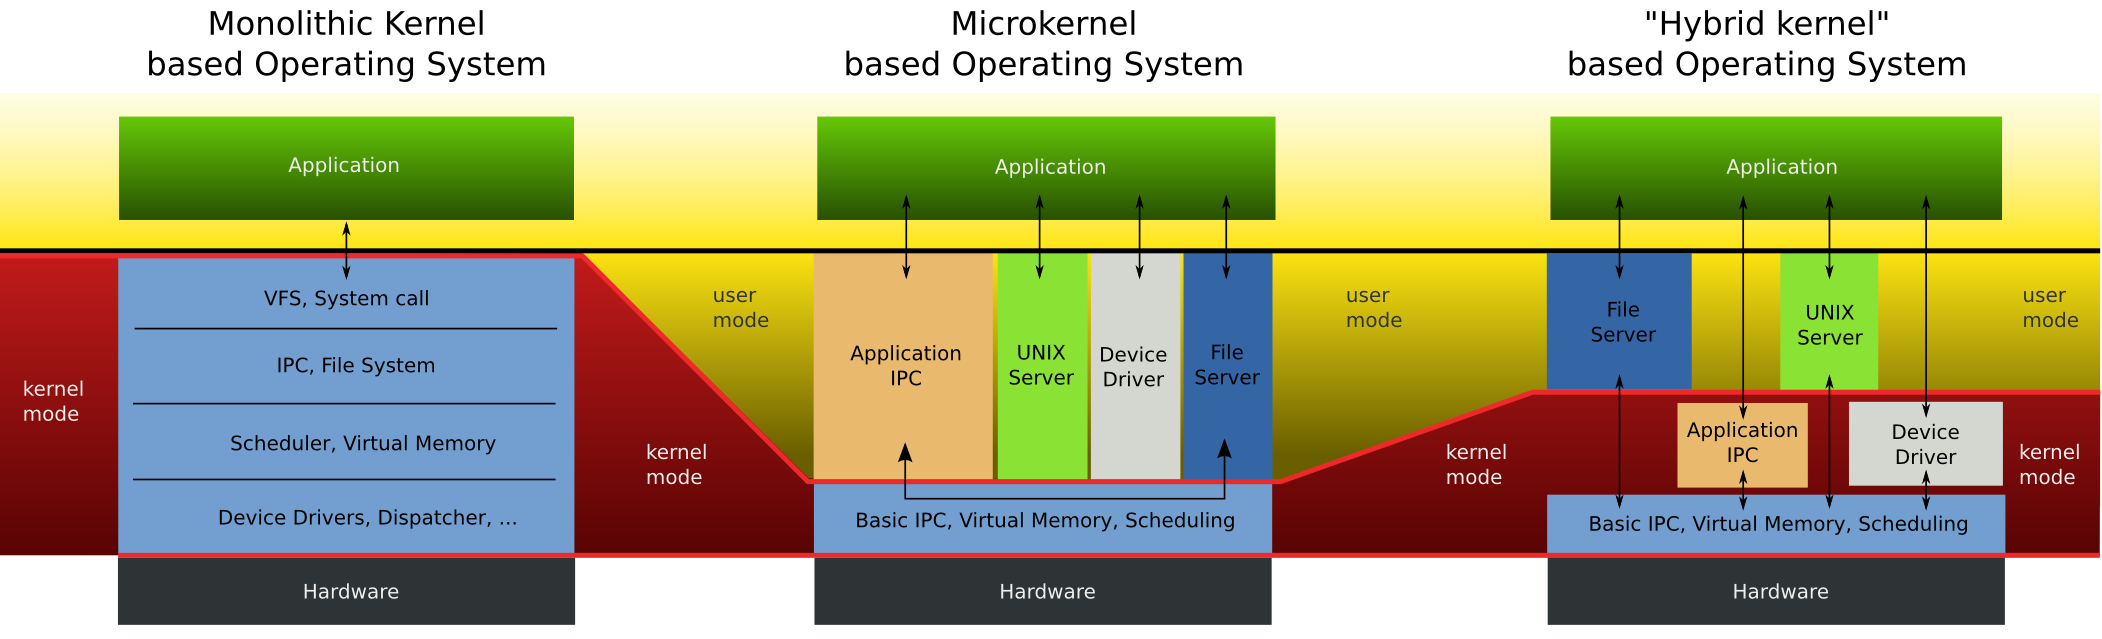
\includegraphics[width=\columnwidth]{OS-structure2.png}    
  \end{center}
\tiny{\url{http://upload.wikimedia.org/wikipedia/commons/d/d0/OS-structure2.svg}}
\end{frame}

\begin{frame} \frametitle{Principales arquitecturas CPU/ports}
  \begin{center}
  \begin{tabular}[center]{|l|cccccc|}
\hline
& WinNT& XNU & Linux& {\color{red}EKA2}\footnote{Symbian}&FreeBSD& {\color{red}WinCE}\\
\hline
\rowcolor[rgb]{1,0.95,0.77}
x86& {\color{verde}\ding{51}} & {\color{verde}\ding{51}} &
{\color{verde}\ding{51}}&{\color{verde}\ding{51}}&
{\color{verde}\ding{51}} & {\color{verde}\ding{51}}\\
\rowcolor[rgb]{1,0.95,0.77}
x86\_64 & {\color{verde}\ding{51}} & {\color{verde}\ding{51}} &
{\color{verde}\ding{51}}& {\color{red}\ding{55}}&
{\color{verde}\ding{51}}& {\color{red}\ding{55}}\\
\rowcolor[rgb]{1,0.95,0.77}
arm & {\color{verde}\ding{51}}&
{\color{verde}\ding{51}}& {\color{verde}\ding{51}}&
{\color{verde}\ding{51}}& {\color{verde}\ding{51}}&
{\color{verde}\ding{51}}\\
\rowcolor[rgb]{1,0.95,0.77}
arm64 & {\color{verde}\ding{51}}&
{\color{verde}\ding{51}}& {\color{verde}\ding{51}}&
{\color{red}\ding{55}}& {\color{verde}\ding{51}}&
{\color{red}\ding{55}}\\
mips &  {\color{red}\ding{55}} & {\color{red}\ding{55}} &
{\color{verde}\ding{51}}& {\color{red}\ding{55}}&
{\color{verde}\ding{51}}&{\color{verde}\ding{51}}\\
powerpc & {\color{red}\ding{55}} &{\color{verde}\ding{51}} &
{\color{verde}\ding{51}}& {\color{red}\ding{55}}&
{\color{verde}\ding{51}}& {\color{red}\ding{55}}\\ 
sparc64& {\color{red}\ding{55}} & {\color{red}\ding{55}}
&{\color{verde}\ding{51}}& {\color{red}\ding{55}}&
{\color{verde}\ding{51}}& {\color{red}\ding{55}}\\ 
alpha & {\color{red}\ding{55}} & {\color{red}\ding{55}} &
{\color{verde}\ding{51}}& {\color{red}\ding{55}}&
{\color{red}\ding{55}} & {\color{red}\ding{55}} \\
ia64 & {\color{red}\ding{55}} & {\color{red}\ding{55}} &
{\color{verde}\ding{51}}& {\color{red}\ding{55}}&
{\color{red}\ding{55}} & {\color{red}\ding{55}}\\
m68k & {\color{red}\ding{55}} & {\color{red}\ding{55}} &
{\color{verde}\ding{51}}& {\color{red}\ding{55}}&
{\color{red}\ding{55}} & {\color{red}\ding{55}}\\
parisc & {\color{red}\ding{55}} & {\color{red}\ding{55}} &
{\color{verde}\ding{51}}& {\color{red}\ding{55}}&
{\color{red}\ding{55}}& {\color{red}\ding{55}}\\ 
sparc & {\color{red}\ding{55}} & {\color{red}\ding{55}} &
{\color{verde}\ding{51}}& {\color{red}\ding{55}}&
{\color{red}\ding{55}}& {\color{red}\ding{55}}\\ 
\hline
  \end{tabular}    
  \end{center}
\end{frame}

\end{document}
